\section{Specification analysis}

\subsection{Algorithm description}
We have implemented an AES S-box based stream cipher supporting both encryption and decryption. As this is a stream cipher, the encryption algorithm is based on a XOR operation of each plaintext character (represented as an 8-bit ASCII coded character) with an 8-bit value of the keystream, which is pseudo-randomly generated.

In this project, we use as a PRBG for the keystream an 8-bit counter which is substituted with the S-box transformation of the AES algorithm. The 8-bit counter (called \textit{Counter Block}) is initialized with the symmetric key $K$. The encryption algorithm can be expressed as follows:
\begin{equation}
    \label{eqn:enc}
    ct[i] = pt[i] \oplus S(cb[i])
\end{equation}
where
\begin{align*}
     & \  ct[i]     &  & \text{is the 8-bit ASCII code of the i\textsuperscript{th} character of ciphertext}                                                                                                                                \\
     & \  pt[i]     &  & \text{is the 8-bit ASCII code of the i\textsuperscript{th} character of plaintext}                                                                                                                                 \\
     & \ cb[i]      &  & \parbox{11cm}{is the 8-bit value of the i\textsuperscript{th} counter (counter block), for $i = 0,1,2, \dots$, and it can be represented by the formula $cb[i] = K + i \mod 256$, being K the 8-bit symmetric key} \\
     & S(\quad )    &  & \parbox{11cm}{is the S-box transformation of the AES algorithm, working over 8-bit values}                                                                                                                         \\
     & \ \ \ \oplus &  & \text{is the XOR operation}                                                                                                                                                                                        \\
\end{align*}

The decryption is performed in the same way of the encryption, where the plaintext and the ciphertext are swapped in the formula, that is:
\begin{equation}
    \label{eqn:dec}
    pt[i] = ct[i] \oplus S(cb[i])
\end{equation}
The proof is very simple and it is based on the associative and self-inverse XOR properties.

\begin{theorem}
    \label{thm:enc_inv_dec}
    Let $ct[i]$ be the result of the encryption of $pt[i]$ as in \cref{eqn:enc} with key $K$, then the result of the decryption of $ct[i]$ with key $K$ as in \cref{eqn:dec} is equal to $pt[i]$.
\end{theorem}

\begin{proof}
    \begin{align*}
        pt[i] & = ct[i] \oplus S(cb[i])                                \\
              & = \left(pt[i] \oplus S(cb[i]) \right) \oplus S(cb[i])  \\
              & = pt[i] \oplus \left(S(cb[i])  \oplus S(cb[i]) \right) \\
              & = pt[i]
    \end{align*}
\end{proof}

\subsection{Additional design specification}
The design module shall encrypt one plaintext (ciphertext) character per clock cycle, and must also feature an asynchronous active-low reset port.
The input data character (either plaintext or ciphertext) can be any 8-bit ASCII character.
To recognize valid inputs and outputs, the module shall have two 1-bit signals ($din\_valid$ for input and $dout\_valid$ for output) that must be asserted (i.e. $1$) when the input/output character is valid and stable, otherwise it must be deasserted (i.e. $0$).

\begin{figure}
    \centering
    \begin{subfigure}{.95\textwidth}
        \centering
        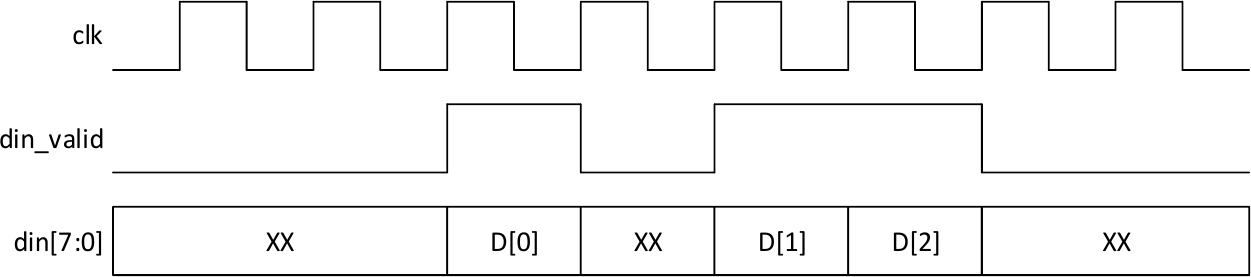
\includegraphics[width=1\textwidth]{din}
        \caption{Input}
        \label{fig:input_expected_waveform}
        \vspace*{.6cm}
    \end{subfigure}
    \begin{subfigure}{.95\textwidth}
        \centering
        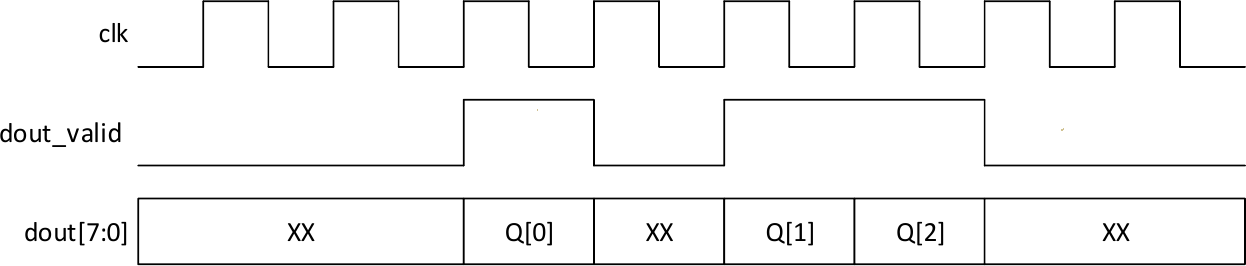
\includegraphics[width=1\textwidth]{dout}
        \caption{Output}
        \label{fig:output_expected_waveform}
    \end{subfigure}
    \caption{Expected waveforms}
    \label{fig:expected_waveforms}
\end{figure}